\chapter{Implémentation}
\label{chap:realisation}

\agtlettrine{L}a conception ayant posé l'architecture et les
comportements attendus du système, ce chapitre décrit sa mise en œuvre
concrète : l'environnement et les outils retenus, la méthodologie de
travail suivie, la réalisation module par module, les difficultés
rencontrées et le déploiement réel de l'outil.
\minisommaire

\section{Environnement et outils de développement}

Les choix technologiques présentés ici ne précèdent pas la conception,
ils en découlent : chaque outil retenu répond à une contrainte déjà
posée au chapitre précédent, plutôt qu'à une préférence de départ.

\subsection{Backend}

\begin{table}[H]
\centering
\renewcommand{\arraystretch}{1.6}
\begin{tabular}{p{1.6cm}p{2.6cm}p{8.6cm}}
\toprule
\textbf{Logo} & \textbf{Technologie} & \textbf{Justification} \\
\midrule

\includegraphics[height=1cm]{assets/icons/04-icone_fastapi.png} &
FastAPI &
Le backend concentre toute vérification RBAC/IBAC à chaque requête et
diffuse plusieurs flux temps réel (journaux, console web). FastAPI
propose nativement les deux : une gestion asynchrone des requêtes et un
support intégré des WebSocket, sans bibliothèque tierce. \\
\addlinespace

\includegraphics[height=1cm]{assets/icons/04-icone_postgresql.png} & PostgreSQL et SQLAlchemy 2.0 &
La base de données relationnelle porte des entités aux relations
riches (utilisateurs, rôles, permissions, portées). Un ORM mature,
compatible avec l'écriture asynchrone de FastAPI, évite d'écrire du SQL
brut pour chaque requête. \\
\addlinespace
(logo non disponible) & Alembic &
Le modèle de données évolue au fil de l'implémentation du projet. Alembic
permet de versionner chaque évolution du schéma sans perte de données
sur un environnement déjà en service. \\
% \addlinespace
% (logo non disponible) & Pydantic v2 &
% Chaque requête et chaque réponse de l'API doivent être validées
% strictement, en particulier pour ne jamais exposer un secret en clair.
% Pydantic valide les schémas de données à l'entrée et à la sortie de
% l'API, avec un typage explicite. \\
\addlinespace
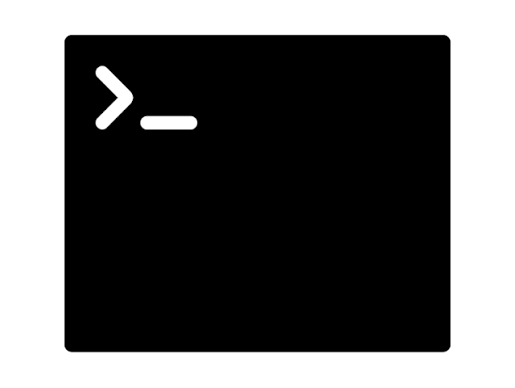
\includegraphics[height=1cm]{assets/icons/04-icone_ssh.png} &
Paramiko &
Toute opération sur un serveur distant passe par un unique adaptateur
SSH, sans agent installé sur les cibles. Paramiko implémente le
protocole SSH directement en Python, sans dépendre d'un client SSH
externe installé sur la machine hôte. \\
\bottomrule
\end{tabular}
\caption{Technologies backend et justification par contrainte de conception}
\end{table}

\subsection{Frontend}

\begin{table}[H]
\centering
\renewcommand{\arraystretch}{1.6}
\begin{tabular}{p{1.6cm}p{2.6cm}p{8.6cm}}
\toprule
\textbf{Logo} & \textbf{Technologie} & \textbf{Justification} \\
\midrule

\includegraphics[height=1cm]{assets/icons/04-icone_react.png} &
React &
L'interface web ne porte aucune logique d'autorisation, mais doit
adapter dynamiquement l'affichage selon les permissions reçues de l'API.
Un modèle par composants facilite ce masquage conditionnel, écran par
écran. \\
\addlinespace
(logo non disponnible) & TypeScript &
L'interface consomme des contrats de données définis côté backend. Le typage statique évite
une classe entière d'erreurs d'intégration entre les deux couches. \\
\addlinespace

\includegraphics[height=1cm]{assets/icons/04-icone_vite.png} &
Vite &
Le développement de l'interface s'est fait par itérations rapprochées,
module par module, tout au long des sessions d'implémentation. Vite réduit le
temps de rechargement à chaque modification, ce qui a compté sur un
développement aussi séquentiel. \\
\addlinespace
(logo non disponible) & Tailwind CSS &
L'interface gère simultanément un mode clair et un mode sombre, avec
une palette sémantique de statuts (succès, erreur, avertissement).
Tailwind permet de centraliser ces jetons de style sans dupliquer de
CSS écran par écran. \\
\bottomrule
\end{tabular}
\caption{Technologies frontend et justification par contrainte de conception}
\end{table}

\subsection{Outils et intégrations transverses}

\begin{table}[H]
\centering
\renewcommand{\arraystretch}{1.6}
\begin{tabular}{p{1.6cm}p{2.6cm}p{8.6cm}}
\toprule
\textbf{Logo} & \textbf{Technologie} & \textbf{Justification} \\
\midrule

\includegraphics[height=1cm]{assets/icons/04-icone_docker.png} &
Docker &
AGT Infra pilote des conteneurs déjà en place chez AG Technologies,
sans réimplémenter de moteur de conteneurisation. Docker est piloté
exclusivement en ligne de commande via SSH, jamais par son API TCP, ce
qui évite d'exposer un port supplémentaire sur chaque serveur. \\
\addlinespace

\includegraphics[height=1cm]{assets/icons/04-icone_git.png}

\includegraphics[height=1cm]{assets/icons/04-icone_github.png} &
Git / GitHub &
Le déploiement continu se déclenche par un évènement webhook signé,
émis par le dépôt du projet à déployer. GitHub héberge ces dépôts et
fournit ce mécanisme de webhook nativement. \\
\addlinespace
(logo non fourni) & Nginx / Certbot &
La publication applicative expose une application déjà déployée, sous
HTTPS, sans que l'outil ne réimplémente de serveur web ni d'autorité de
certification. Nginx et Certbot, pilotés par SSH comme le reste,
couvrent ce besoin sans nouvelle dépendance sur les serveurs cibles. \\
\addlinespace

\includegraphics[height=1cm]{assets/icons/04-icone_netdata.png} &
Netdata &
La supervision continue repose sur un agent autonome, installé une
seule fois manuellement, capable de notifier l'API backend par webhook
en cas de dépassement de seuil, indépendamment de toute consultation en
cours. \\
\bottomrule
\end{tabular}
\caption{Outils et intégrations transverses}
\end{table}




\section{Méthodologie de travail}

La réalisation du projet s'est étalée sur plusieurs sessions successives, chacune portant sur
un domaine fonctionnel précis. Cet étalement a rendu nécessaire une
méthodologie de travail rigoureuse, tant pour garantir la qualité de
chaque livraison que pour assurer la continuité.

\subsection{Cycle de développement}

Chaque évolution du projet, qu'il s'agisse d'un nouveau module ou d'une
correction, a suivi un cycle en quatre étapes, appliqué sans exception :

\begin{enumerate}
  \item \textbf{Audit} : avant toute modification, un état des lieux du
        code existant concerné est établi, afin d'en comprendre la structure et les relations avant d'y intervenir.
  \item \textbf{Plan et/ou maquette UI} : un plan de travail est défini, précisant les
        changements à apporter et leur impact attendu sur le reste du
        système, avant toute écriture de code.
  \item \textbf{Implémentation} : le plan une fois arrêté, les
        changements sont mis en œuvre.
  \item \textbf{Test} : chaque changement est ensuite vérifié, afin de
        s'assurer qu'il fonctionne comme attendu et qu'aucune
        fonctionnalité existante n'a été affectée.
\end{enumerate}

Ce cycle a permis d'éviter un écueil fréquent dans un projet de cette
ampleur : coder avant d'avoir complètement cerné l'impact d'un
changement sur des modules déjà en place, en particulier pour le
contrôle d'accès, dont une régression aurait pu affecter l'ensemble du
système.

\subsection{Traçabilité des décisions}

Toute décision d'architecture prise pendant le projet est numérotée, 
de même que tout bogue identifié. Cette numérotation continue permet de retrouver, à tout
moment, la justification d'un choix technique précis sans avoir à
reconstituer son historique de mémoire.

\subsection{Continuité}

Le projet s'étalant sur plusieurs sessions d 'implémntation, sa continuité repose sur un
petit ensemble de documents tenus à jour :

\begin{itemize}
  \item Un journal de session, décrivant ce qui a été réalisé et ce qui
        reste en suspens.
  \item Une liste de tâches, corrigée à la fin de chaque session plutôt
        que laissée à reconstituer au début de la suivante.
  \item Un index recensant, session après session, ce qui a été livré.
\end{itemize}

Cette organisation a permis de reprendre chaque session de travail sans
perte d'information et devoir refaire un audit complet, malgré l'étalement du projet sur plusieurs semaines
et l'intervention de plusieurs domaines fonctionnels en parallèle.

\bigskip
\noindent\textit{Note : une partie de ce cycle de développement,
notamment la relecture de code existant, a été accélérée par l'usage d'un assistant d'intelligence
artificielle, sous la supervision et la validation systématique de
l'auteur à chaque étape.}




\section{Réalisations par module}

Cette section détaille cinq modules fonctionnels. Pour chacun, le
fonctionnement technique réel est décrit (mécanismes, algorithmes,
protocoles), sans extrait de code, ainsi que l'état d'avancement et les
limites connues à ce jour.

\subsection{Gestion des serveurs et des conteneurs Docker}

\textbf{Connectivité SSH.} Le branchement d'un serveur s'authentifie par
mot de passe ou par une paire de clés générée individuellement pour ce
serveur. L'adaptateur SSH détecte automatiquement le format de la clé
privée fournie (RSA, Ed25519, ECDSA ou DSA) en tentant successivement
chaque analyse jusqu'à obtenir une clé exploitable. La clé privée est
chiffrée avant stockage et n'est jamais restituée en clair par l'API,
y compris pour le rôle disposant d'un accès total.

\textbf{Cycle de vie d'une demande de clé dédiée.} Lorsqu'une clé
dédiée est demandée plutôt qu'un mot de passe, une paire est générée et
seule la clé publique est affichée, accompagnée d'un délai
d'installation configurable. Si la clé publique n'est pas installée sur
le serveur avant l'expiration de ce délai, la demande est invalidée et
son secret associé supprimé, sans action manuelle.

\textbf{Conteneurs et registres.} Docker est piloté par des commandes
exécutées en ligne de commande via SSH, jamais par son API TCP native,
ce qui évite d'exposer un port ou un socket Docker supplémentaire sur
chaque serveur. Un registre de conteneurs privé peut être enregistré
par utilisateur ; son secret d'accès suit le même principe de
chiffrement au repos et de non-exposition que les clés SSH.

\textbf{Console web.} L'ouverture d'une session sur un serveur ouvre un
canal interactif direct sur la machine distante. Sur un conteneur, la
session ouvre d'abord un canal SSH classique, puis y exécute une
commande d'attachement interactif au conteneur ciblé, ce qui donne
l'illusion d'une session directe sans exposer d'accès SSH séparé au
conteneur lui-même. Le flux complet de chaque session, entrées et
sorties confondues, est écrit ligne par ligne dans un fichier structuré,
consultable ensuite par relecture intégrale.

\subsection{Déploiement continu}

\textbf{Déclenchement.} Un déploiement démarre soit par un évènement
webhook GitHub, soit manuellement depuis l'interface. Dans le premier
cas, la charge utile reçue est vérifiée par une signature HMAC-SHA256
calculée à partir d'un secret propre à la configuration ; toute
signature invalide entraîne un rejet immédiat, avant toute autre
vérification.

\textbf{Moteur d'exécution.} Aucune file de tâches externe n'est
utilisée : chaque déploiement s'exécute comme une tâche asynchrone du
serveur applicatif lui-même. Un verrou au niveau de la base de données,
propre à chaque configuration, empêche deux déploiements concurrents sur
la même configuration. Au démarrage du service, les exécutions restées
bloquées à l'état "en cours" à la suite d'un arrêt inattendu sont
détectées et réconciliées, plutôt que laissées indéfiniment ouvertes.

\textbf{Séquence de phases.} Chaque déploiement traverse les phases
suivantes, dans un ordre strict :

\begin{enumerate}
  \item connexion SSH au serveur cible ;
  \item vérifications préalables (précondition), avec possibilité
        d'exécution à blanc ;
  \item synchronisation du dépôt Git, conçue pour être rejouée sans
        effet différent si elle est répétée ;
  \item génération du fichier de variables d'environnement, à partir de
        secrets déchiffrés au moment de l'exécution seulement ;
  \item construction de l'image et démarrage du conteneur ;
  \item vérification de bon fonctionnement du conteneur démarré ;
  \item nettoyage des ressources temporaires laissées par la
        construction.
\end{enumerate}

Un échec à l'étape de vérification de bon fonctionnement déclenche un
retour arrière automatique vers le dernier conteneur connu comme stable.

\textbf{Journalisation.} Chaque phase écrit sa progression dans un
fichier \textbf{jsonl} détaillé sur disque, diffusé simultanément en direct sur un
canal WebSocket dédié. Une synthèse de l'exécution (résultat, durée,
commit, acteur) est écrite séparément en base de données : la
suppression ultérieure du fichier détaillé, lors d'une purge, ne fait
donc pas disparaître cette synthèse. Cette méthode combinée évite de
saturer la base de données avec un volume de texte potentiellement
important, tout en conservant une trace consultable de chaque
exécution.

\subsection{Publication applicative}

\textbf{Préconditions.} Une publication ne peut être créée que pour une
configuration de déploiement ayant déjà connu au moins une exécution
réussie, et associée à un conteneur du même serveur. La résolution DNS
du domaine visé est vérifiée avant toute configuration du serveur ;
aucun enregistrement DNS n'est créé par l'outil lui-même.

\textbf{Configuration du proxy (Nginx) et de cerbot.} La configuration du serveur web et la
demande de certificat HTTPS cerbotsont générées puis appliquées sur le
serveur cible via SSH. Le port cible d'une route est proposé
automatiquement à partir du port réel exposé par le conteneur ou la
configuration associée, mais reste modifiable avant confirmation.

\textbf{Détection d'incohérence.} Une fois active, une publication est
périodiquement confrontée à l'état réel de sa cible (port, conteneur
associé). Toute incohérence détectée fait passer la publication à
l'état désynchronisée, sans correction automatique : seule une action
volontaire de l'utilisateur permet de sortir de cet état.


\subsection{Supervision continue}

\textbf{Bootstrap.} L'agent de supervision est installé manuellement
une seule fois sur chaque serveur. Sa configuration réseau est fixée en
constante côté code pour n'écouter que sur l'interface locale de la
machine, jamais accessible à distance directement : c'est AGT Infra qui
vient chercher les métriques, pas l'inverse.

\textbf{Double canal.} Deux flux distincts existent. Le premier est une
notification autonome : lorsqu'un seuil est dépassé, l'agent envoie un
webhook, vérifié par une signature selon le même principe que le
webhook de déploiement. Le second est un flux de consultation en
direct : un tunnel SSH est ouvert vers le port local de l'agent, puis
relayé à l'interface par un canal WebSocket, ce qui donne accès aux
métriques en direct sans jamais exposer le port de l'agent sur le
réseau public du serveur.

\textbf{Seuils personnalisés.} Une surcharge de seuils par serveur est
écrite dans un fichier de configuration dédié, distinct des fichiers
natifs de l'agent, afin de ne jamais écraser un réglage existant qui ne
relèverait pas d'AGT Infra. Un changement de collecteurs actifs déclenche
un redémarrage complet de l'agent, tandis qu'un changement limité aux
seuils ou aux canaux de notification ne déclenche qu'un rechargement
partiel, plus rapide et moins intrusif.

\textbf{Filtrage des métriques.} Le flux de métriques brutes de l'agent
étant disproportionné pour un usage direct, seules les valeurs
correspondant aux collecteurs activés pour ce serveur sont retenues et
transmises à l'interface.

\subsection{Contrôle d'accès (RBAC/IBAC)}

\textbf{Modèle de données.} Les rôles et les permissions ne pas
des valeurs fixes définies dans le code, mais des enregistrements en
base de données, librement composables depuis l'interface. Seul le rôle
disposant d'un accès total reste immuable et non supprimable.

\textbf{Algorithme de résolution.} Chaque requête sensible déclenche une
vérification qui suit l'ordre déjà détaillé au
chapitre~\ref{chap:etude-technique} : accès immédiat pour le rôle
immuable, puis recherche d'un refus direct, puis d'une autorisation
directe, puis d'une autorisation via un rôle, avec un refus par défaut
si aucune de ces conditions n'est remplie. \\ 
Cette vérification est appliquée de façon uniforme sur les routes classiques comme sur les
connexions WebSocket, ces dernières étant authentifiées par un jeton
transmis en paramètre de connexion plutôt que par un en-tête classique.

\textbf{Filtrage par ressource.} Sur les listes de serveurs, de
conteneurs et de configurations de déploiement, la liste retournée est
désormais restreinte aux seules ressources auxquelles la personne a
effectivement accès, plutôt que retournée en entier puis filtrée à
l'affichage. Une personne sans permission de lecture globale reçoit
ainsi une liste vide plutôt qu'un refus d'accès, ce qui reste cohérent
avec une consultation partielle légitime via des permissions restreintes
à certaines ressources.

\section{Difficultés rencontrées et solutions apportées}

\subsection{Absence d'environnement de test représentatif}

\begin{itemize}
  \item \textbf{Constat} : le développement ne pouvait pas s'appuyer sur
        les serveurs de production de l'entreprise, qui hébergent des
        applications réelles et ne pouvaient pas être exposés à un
        risque d'instabilité.
  \item \textbf{Solution apportée} : cette constrainte a été contourné en
        combinant un VPS Hostinger propre à l'entreprise et plusieurs
        machines virtuelles créées sous VirtualBox, ce qui a permis de
        tester librement la connectivité SSH, le déploiement et la
        supervision sans dépendre d'une infrastructure de production.
\end{itemize}

\subsection{Montée en charge du périmètre en cours de stage}

\begin{itemize}
  \item \textbf{Constat} : la mission confiée portait initialement sur
        la prise en main d'outils existants, avant de porter sur ce qui
        est devenu AGT Infra. Le périmètre du projet a ensuite continué
        de s'étendre au fil des sessions, avec l'apparition de domaines
        entiers non prévus au départ (publication applicative,
        supervision continue).
  \item \textbf{Solution apportée} : cette évolution a nécessité de
        revoir la feuille de route à plusieurs reprises plutôt que de
        suivre un plan figé dès le premier jour.
\end{itemize}

\subsection{Remise en cause d'un choix de conception déjà en place}

\begin{itemize}
  \item \textbf{Constat} : le contrôle d'accès reposait initialement sur
        un nombre fixe de rôles, codés en dur. Ce modèle s'est révélé
        trop rigide face au besoin réel.
  \item \textbf{Solution apportée} : cela a conduit à une refonte
        complète vers un système entièrement piloté en base de données,
        en reprenant du code déjà écrit et validé plutôt qu'en
        l'ajoutant en périphérie.
\end{itemize}

\subsection{Coordination de plusieurs systèmes externes}

\begin{itemize}
  \item \textbf{Constat} : le fonctionnement d'un module donné dépend
        souvent de plusieurs briques externes à la fois (SSH, Docker,
        GitHub, Nginx/Certbot, l'agent de supervision), dont le
        comportement réel devait être observé en pratique plutôt que
        déduit de leur seule documentation.
  \item \textbf{Solution apportée} : isoler chaque intégration derrière
        un adaptateur dédié a permis de circonscrire cette complexité,
        brique par brique, plutôt que de la laisser se propager dans le
        reste du code.
\end{itemize}
\section{Déploiement}

AGT Infra est entièrement conteneurisé, à la fois côté backend et côté
frontend, ce qui lui permet d'être installé sur n'importe quel serveur
disposant de Docker, sans dépendre d'un hébergeur ou d'une configuration
particulière.

\begin{figure}[H]
  \centering
  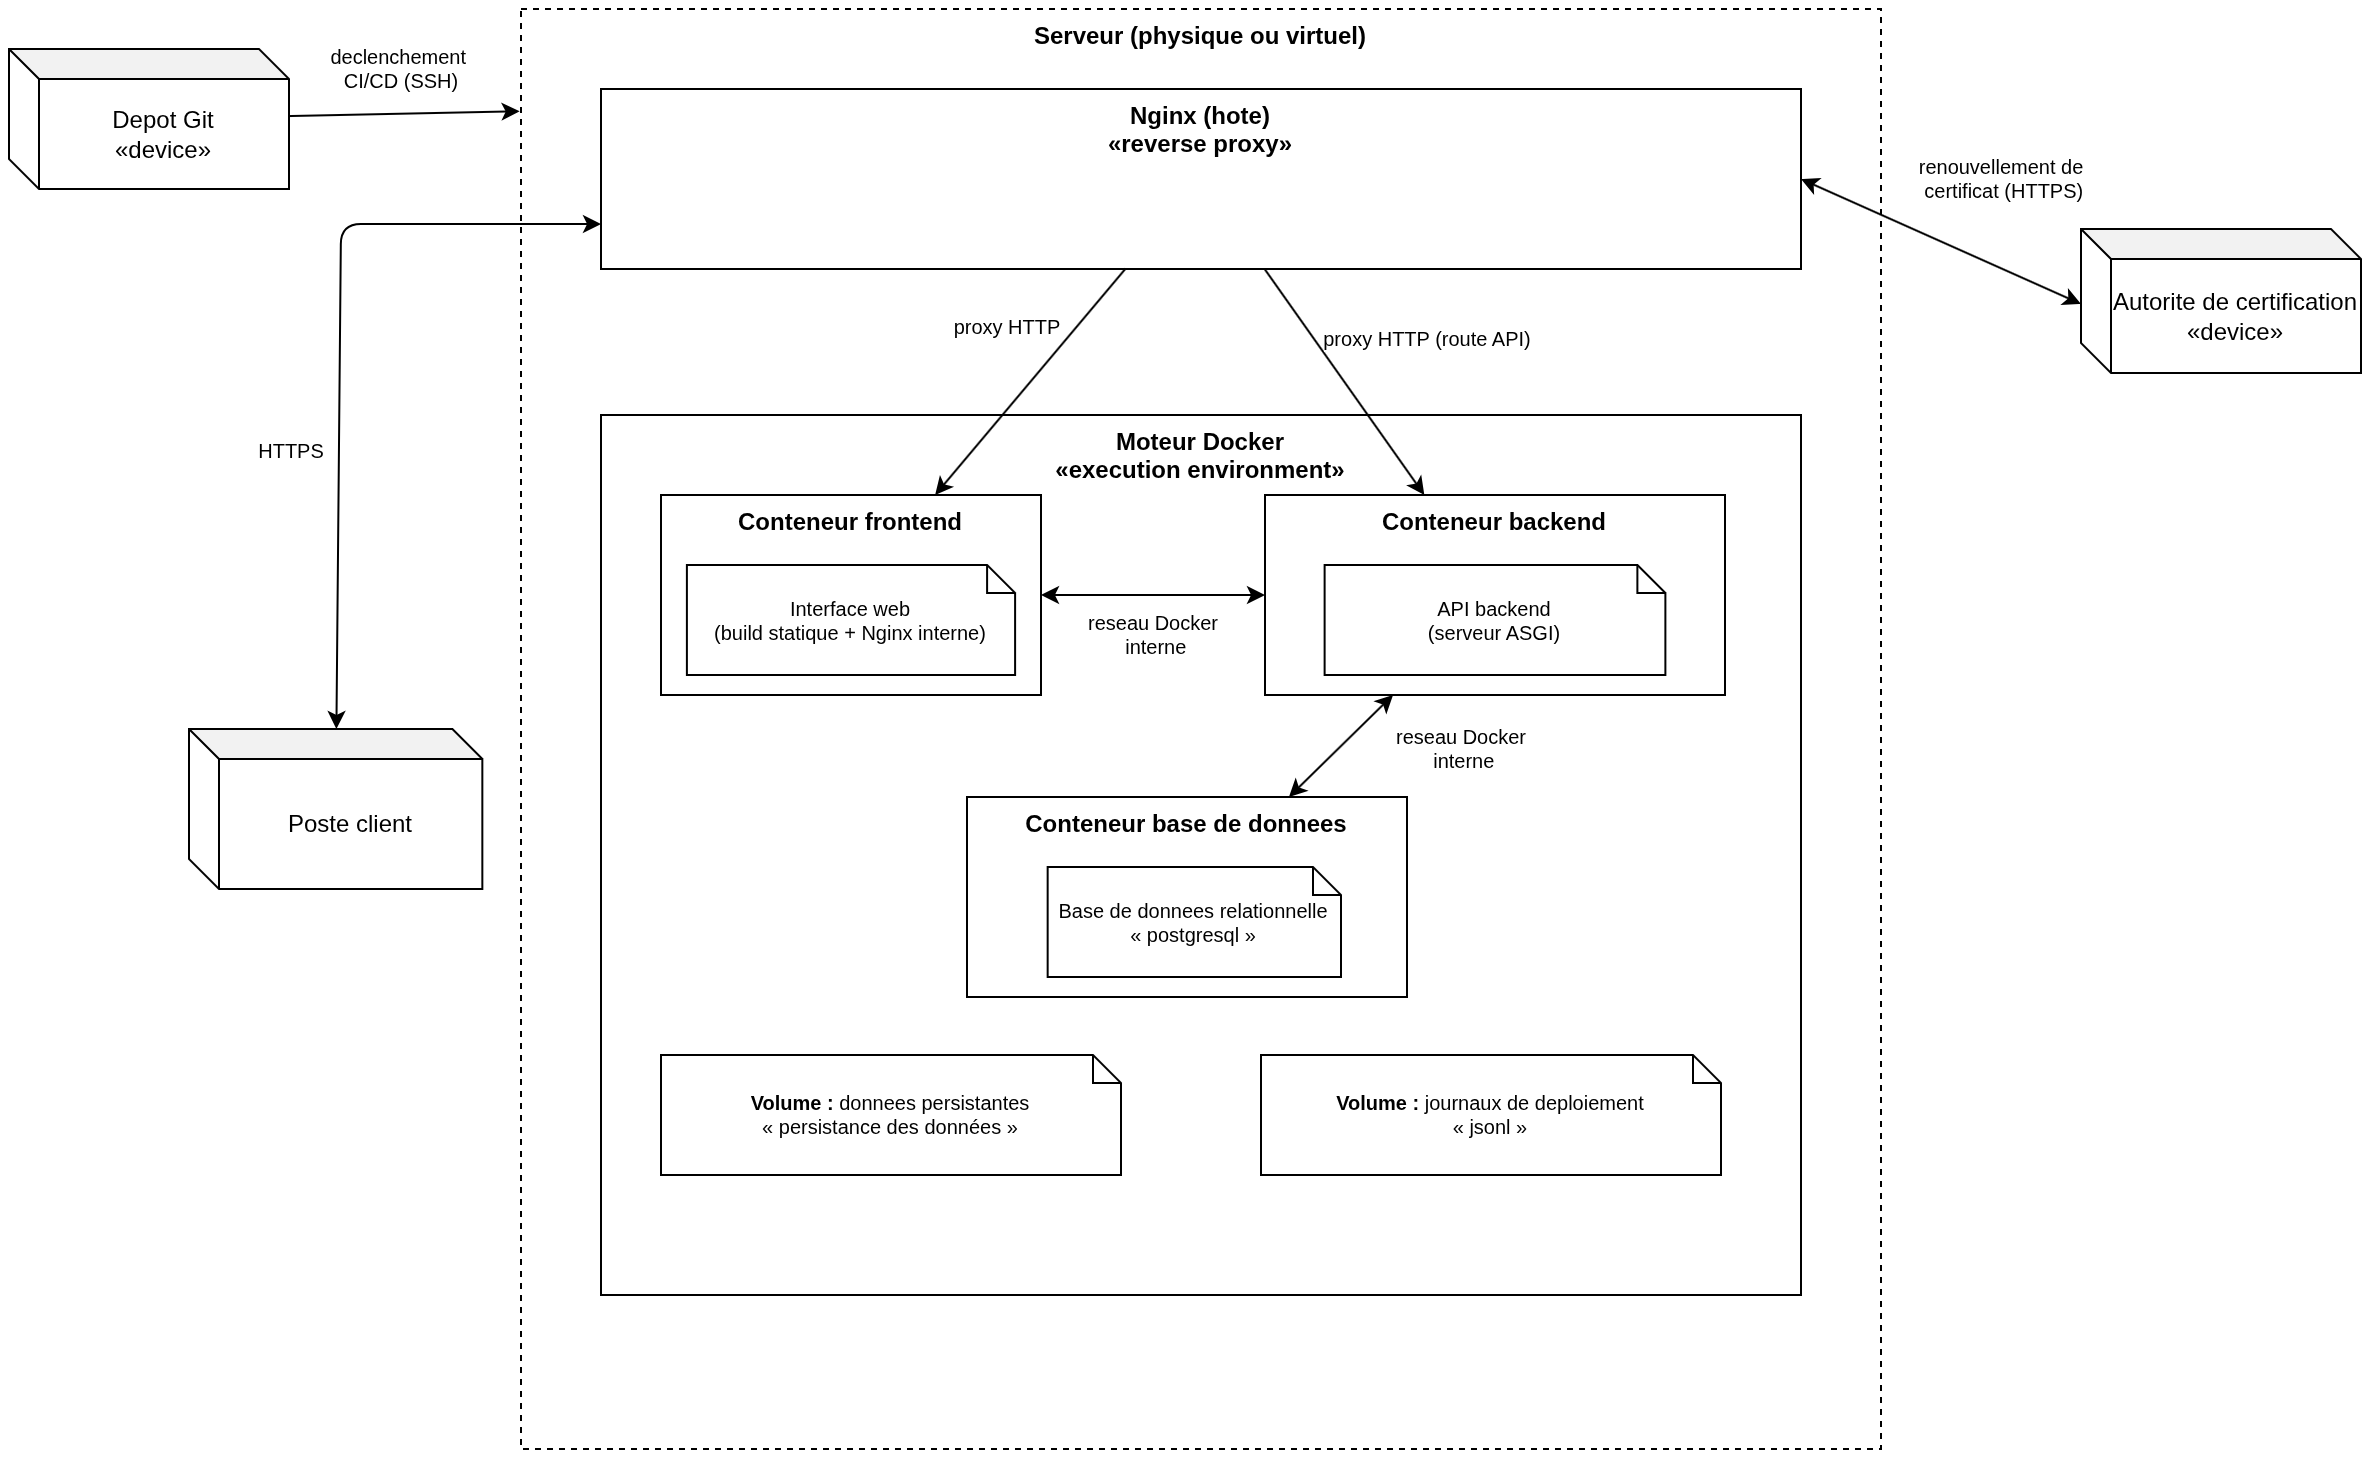
\includegraphics[width=\linewidth]{assets/diagrams/04-diagramme_deploiement.png}
  \caption{Diagramme de déploiement d'AGT Infra}
  \label{fig:diagramme-deploiement}
\end{figure}

Trois conteneurs composent la stack applicative : le frontend (build
statique servi par un Nginx interne au conteneur), le backend (serveur
ASGI exposant l'API) et la base de données relationnelle. Un Nginx
installé directement sur l'hôte, hors de Docker, joue le rôle de
reverse proxy : il reçoit le trafic HTTPS entrant et le redirige vers le
conteneur concerné selon le chemin demandé. Deux volumes Docker assurent
la persistance : l'un pour les données de la base, l'autre pour les
journaux de déploiement. Le renouvellement du certificat HTTPS est
délégué à une autorité de certification externe, et chaque mise à jour
du code est déclenchée par le dépôt Git via une connexion SSH dédiée.

\subsection{Procédure de déploiement}

La procédure suivante reste valable sur tout serveur cible disposant de
Docker, Docker Compose et Nginx. Les valeurs entre chevrons sont propres
à chaque installation.

\begin{enumerate}
  \item \textbf{Cloner le dépôt sur le serveur cible.}
\begin{lstlisting}
mkdir -p ~/apps/agt-infra && cd ~/apps/agt-infra
git clone https://github.com/<compte>/agt-infra.git
cd agt-infra
\end{lstlisting}

  \item \textbf{Vérifier la disponibilité des ports prévus}, en
        particulier sur un serveur déjà utilisé par d'autres projets.
\begin{lstlisting}
docker ps --format '{{.Names}}\t{{.Ports}}'
sudo ss -tlnp | grep -E ':(<port_backend>|<port_frontend>)'
\end{lstlisting}

  \item \textbf{Configurer le reverse proxy Nginx} sur l'hôte, pour le
        nom de domaine visé, avec une redirection vers les deux
        conteneurs.
\begin{lstlisting}
sudo nano /etc/nginx/sites-available/<nom_domaine>
sudo nginx -t
\end{lstlisting}

  \item \textbf{Démarrer la stack applicative}, en combinant la
        configuration commune et la configuration de production
        (ports restreints à l'hôte local, redémarrage automatique).
\begin{lstlisting}
docker compose -f docker-compose.yml -f docker-compose.prod.yml \
  up -d --build
\end{lstlisting}

  \item \textbf{Recharger le reverse proxy} pour prendre en compte la
        nouvelle configuration.
\begin{lstlisting}
sudo systemctl reload nginx
\end{lstlisting}

  \item \textbf{Vérifier que chaque conteneur répond}, avant tout accès
        externe.
\begin{lstlisting}
docker compose -f docker-compose.yml -f docker-compose.prod.yml ps
curl -s http://127.0.0.1:<port_backend>/health
curl -sI http://127.0.0.1:<port_frontend>/
\end{lstlisting}

  \item \textbf{Tester l'accès public sous le nom de domaine}, une fois
        le certificat HTTPS émis.
\begin{lstlisting}
curl -sI https://<nom_domaine>
\end{lstlisting}
\end{enumerate}

\subsection{Redéploiement continu}

Une fois cette bascule initiale effectuée, tout push sur la branche
principale du dépôt déclenche automatiquement un redéploiement, sans
intervention manuelle : une clé SSH dédiée au déploiement, distincte de
toute clé personnelle, autorise le serveur à recevoir cette connexion.
Un script de redéploiement reste disponible en secours, pour le cas où
ce déclenchement automatique échouerait :

\begin{lstlisting}
ssh <utilisateur>@<serveur>
cd ~/apps/agt-infra/agt-infra
./deploy.sh
\end{lstlisting}